\documentclass[landscape]{article}
\usepackage[a4paper, margin=1cm]{geometry}
\usepackage{tikz}
\usetikzlibrary{shapes,arrows,positioning,fit,backgrounds,matrix,decorations.pathreplacing}

\begin{document}

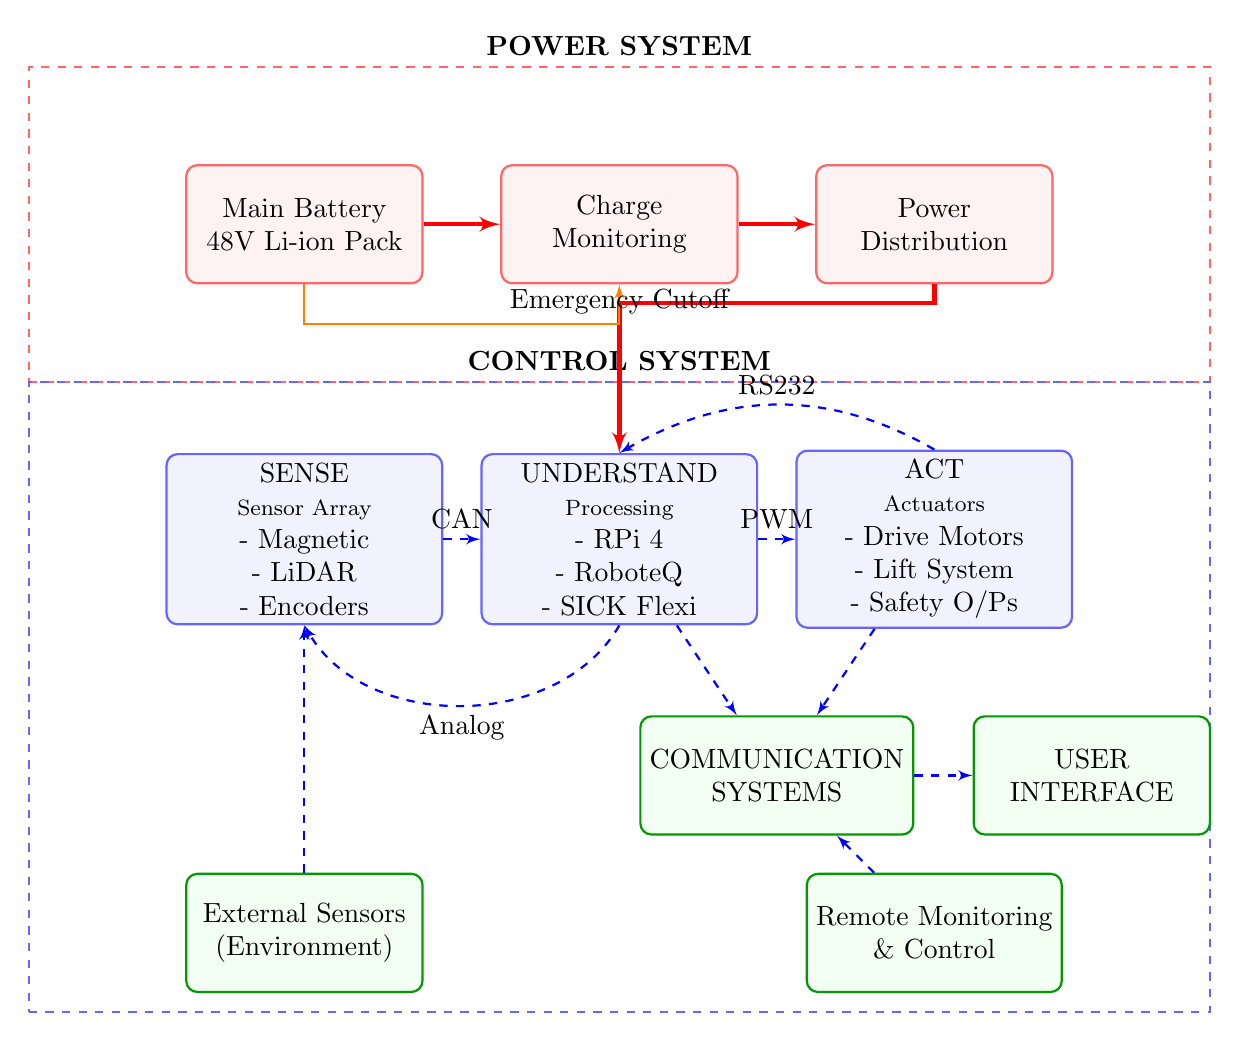
\begin{tikzpicture}[
    auto,
    % Block styles
    powerblock/.style={
        rectangle, 
        draw=red!60, 
        thick,
        fill=red!5,
        minimum height=1.5cm,
        minimum width=3cm,
        align=center,
        rounded corners
    },
    controlblock/.style={
        rectangle,
        draw=blue!60,
        thick,
        fill=blue!5,
        minimum height=2cm,
        minimum width=3.5cm,
        align=center,
        rounded corners
    },
    safetyblock/.style={
        rectangle,
        draw=orange!60,
        thick,
        fill=orange!5,
        minimum height=1.5cm,
        minimum width=3cm,
        align=center,
        rounded corners
    },
    interfaceblock/.style={
        rectangle,
        draw=green!60!black,
        thick,
        fill=green!5,
        minimum height=1.5cm,
        minimum width=3cm,
        align=center,
        rounded corners
    },
    line/.style={draw, thick, -latex'},
    dataline/.style={draw=blue, thick, dashed, -latex'},
    powerline/.style={draw=red, ultra thick, -latex'},
    safetyline/.style={draw=orange, thick, -latex'}
]

% Power System Layer
\node[draw=red!60, thick, dashed, minimum width=15cm, minimum height=4cm] (power_system) at (0,6) {};
\node[above] at (power_system.north) {\textbf{POWER SYSTEM}};

\node[powerblock] (battery) at (-4,6) {Main Battery\\48V Li-ion Pack};
\node[powerblock] (charging) at (0,6) {Charge\\Monitoring};
\node[powerblock] (distribution) at (4,6) {Power\\Distribution};

% Control System Layer
\node[draw=blue!60, thick, dashed, minimum width=15cm, minimum height=8cm] (control_system) at (0,0) {};
\node[above] at (control_system.north) {\textbf{CONTROL SYSTEM}};

\node[controlblock] (sense) at (-4,2) {SENSE\\
    \footnotesize
    Sensor Array\\
    - Magnetic\\
    - LiDAR\\
    - Encoders};

\node[controlblock] (understand) at (0,2) {UNDERSTAND\\
    \footnotesize
    Processing\\
    - RPi 4\\
    - RoboteQ\\
    - SICK Flexi};

\node[controlblock] (act) at (4,2) {ACT\\
    \footnotesize
    Actuators\\
    - Drive Motors\\
    - Lift System\\
    - Safety O/Ps};

\node[interfaceblock] (ui) at (6,-1) {USER\\INTERFACE};
\node[interfaceblock] (comm) at (2,-1) {COMMUNICATION\\SYSTEMS};

% External Systems
\node[interfaceblock] (ext_sensors) at (-4,-3) {External Sensors\\(Environment)};
\node[interfaceblock] (remote) at (4,-3) {Remote Monitoring\\{\&} Control};

% Connections
\draw[powerline] (battery) -- (charging);
\draw[powerline] (charging) -- (distribution);
\draw[powerline] (distribution) -- ++(0,-1) -| (understand);

\draw[dataline] (sense) -- node[above] {CAN} (understand);
\draw[dataline] (understand) -- node[above] {PWM} (act);
\draw[dataline] (understand) -- (comm);
\draw[dataline] (act) -- (comm);
\draw[dataline] (comm) -- (ui);

% Feedback loops
\draw[dataline] (act.north) to[out=150, in=30] node[above] {RS232} (understand.north);
\draw[dataline] (understand.south) to[out=240, in=300] node[below] {Analog} (sense.south);

% External connections
\draw[dataline] (ext_sensors) -- (sense);
\draw[dataline] (remote) -- (comm);

% Emergency cutoff
\draw[safetyline] (battery.south) -- ++(0,-0.5) -| node[above] {Emergency Cutoff} (charging.south);

\end{tikzpicture}

\end{document}